
\section{The \app Framework Overview}

\begin{figure*}[tbp] \centering
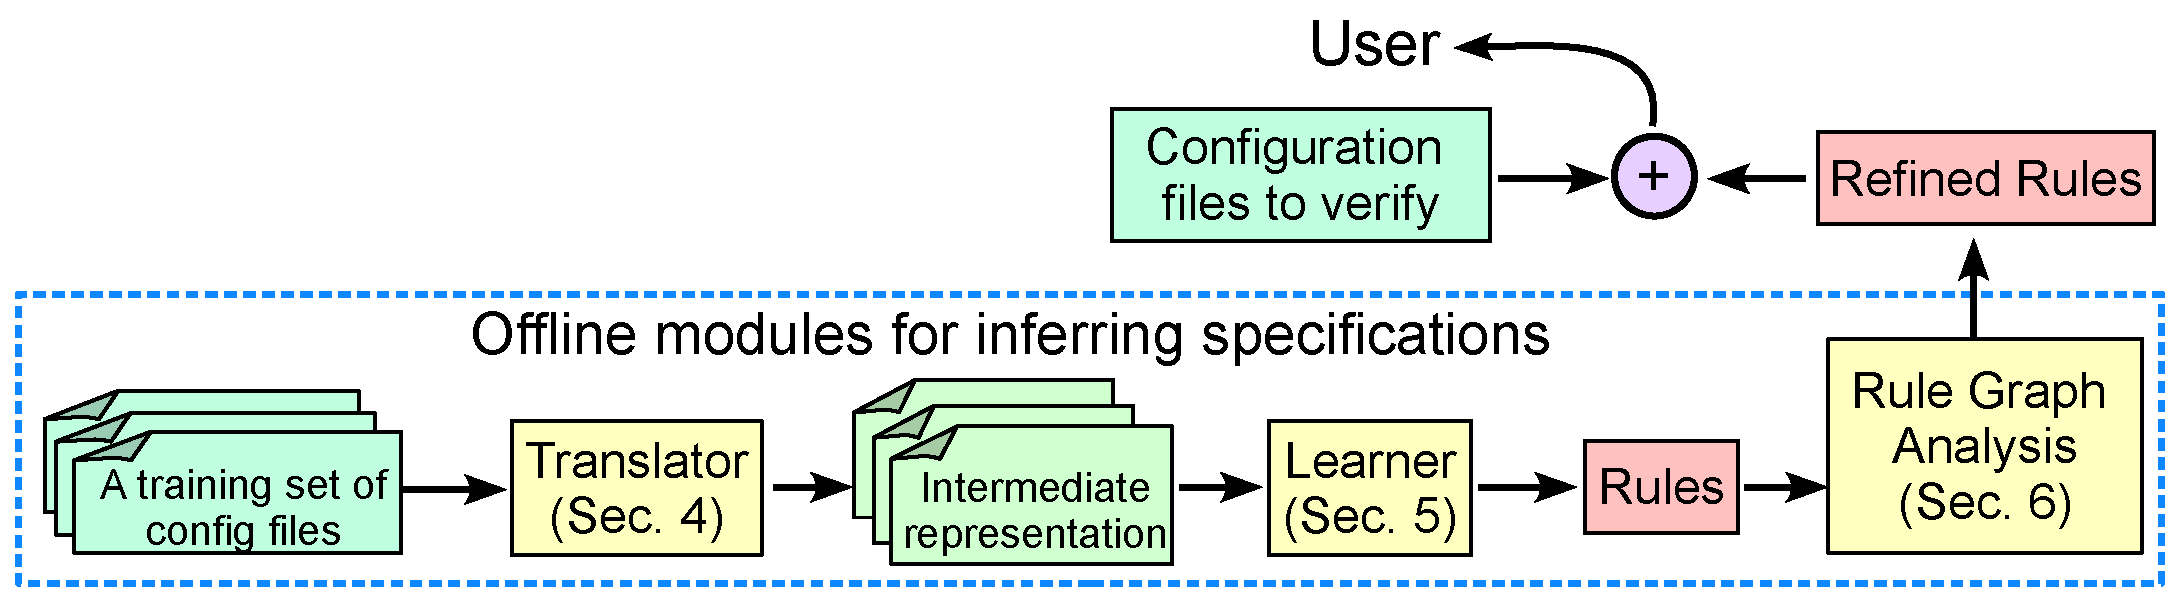
\includegraphics[width=0.99\textwidth]{figs/overview}
\caption{\app's workflow.
  The dashed box is the specification learning module. 
  The yellow components are key modules of \app.}
\label{fig-overview}
\end{figure*}

Figure~\ref{fig-overview} gives an overview of the \app framework.
The biggest part is dedicated to 
learning and inferring the specification for configuration 
files. This process is done offline, before the user even starts 
to use \app. There are three main steps in the process:
translation, learning, and rule refinement.

\para{Initial phase}
Since there is no proper formal specification for configuration 
files, we learn the specification from a large number of 
(not necessarily correct) configuration files belonging to the same 
system, such as MySQL or Apache. These files are our training set.

%In the following steps,
%we will exploit in a collection of learning algorithms 
%to build rules that describe a language model for the files.

\para{Translator}
The translator module first parses the input training  
set of configuration files, and then transforms them into 
a more structured and typed intermediate representation.
Most of entries in a configuration file follow a key-value pattern, 
where some environmental variable (``key'') is assigned  a value.
Looking at a single entry, by inspecting the value
we cannot always fully determine the type of the key~\cite{xu15hey}.
We address this problem 
by introducing {\em probabilistic types}.
Rather than giving a variable a single type, 
we assign several types over a probability distribution. 

\para{Learning}
The learner reads a set of configuration files that have been translated
into well-structured representations. 
It employs a learning algorithm, {\em rule association 
algorithm}, to generate a list of rules, describing properties 
of configuration files. In a nutshell, the learning algorithm 
takes a set of rule interfaces and instantiate them with the concrete
values that appear in the training set. Since there are no guarantees 
that the files in the training set are correct, our main assumption
is that even if a file contains an error, majority of the files do not 
have the same error and our learning process should detect these

generate concrete instances of t

\ruzica{i need to read the rest of the paper first}


These rules are the outputs of the learner, 
and will be used to detect errors later.
Because the translator gives the learner probabilistically typed entries,
the learner is also responsible for determining types for these entries.

\para{Post Analysis}
Finally, the logically structured representation of learned rules allows for a further post analysis stage.
This novel extension infers knowledge on the accepted rules that can improve the output of the system.
As a case study, we build a graph to model the learned rules.
We analyze the properties of this graph to construct an ordering of rules by their importance, 
  as well as to produce a measure of complexity for any configuration of the target system.
While the metrics in used in \app are effective, they are not intended to be exhaustive.
The information contained in the structured representation of the learned rules, 
  is a unique benefit of the learning algorithm, as contrasted with other machine learning techniques.

